\section{\texorpdfstring{Event selection for the \leptonTau channel}{Event selection for the lepton-tau channel}}
\label{sect:eleTauCuts}
Events in the \leptonTau final states (e\Tau and $\mu\Tau$)
are collected with triggers that require 
a loosely isolated \Tau with \PT $>$ 20\GeV and $|\eta|$ $<$ 2.3 as well as
an isolated electron\cite{Khachatryan:2015hwa} or muon\cite{Chatrchyan:2012xi} with $|\eta| < 2.1$.  The minimum
\PT requirement for the electron (muon) was increased during the data taking from 20 to 22\GeV (17 to 18\GeV)
due to the increase in instantaneous luminosity.

In the offline analysis, the electron, muon, and \Tau objects are required to have \PT $>$ 25, 20, and 25\GeV, respectively, 
and the corresponding identification and isolation are tightened.
In events with more than one opposite-sign \leptonTau pair, we only consider
 the pair that maximizes the scalar sum of \Tau and electron or muon 
transverse momenta.  Events with an additional loosely isolated lepton
with \PT $>$ 10\GeV are rejected to suppress backgrounds from $Z$ boson
decays.  

Just as for the \tauTau channel, we apply preselection requirements to suppress
QCD multijet, \ttbar, $Z \to \tau \tau$, and low mass resonance events.
These requirements are: \mttwo $>$ 40\GeV, \MPT $>$ 30\GeV, \leptonTau 
invariant mass between 15 and 45\GeV or $>$ 75\GeV, \deltaphi $>$ 1. We reject events with b-tagged jets.
The final signal region requirements are \mttwo $>$ 90\GeV and 
\tauMT $>$ 200\GeV. %where \tauMT is the \Tau transverse mass 
The latter requirement provides discrimination against the \wjets background.  Unlike the \tauTau channel,
events with \mttwo $<$ 90\GeV are not used because of the higher 
level of background. Table \ref{Tab.Cuts}
\begin{table}[!htb]
\begin{center}
\caption{Definition of signal regions.}
\begin{tabular}{|c|c|c|}
\hline\hline
               & \tauTau & \tauTau               \\
   \leptonTau  & \binone & \bintwo               \\\hline\hline
 OS \leptonTau & \multicolumn{2}{c|}{OS \tauTau}  \\\hline
\multicolumn{3}{|c|}{\MPT $>$ 30\GeV}            \\\hline
\multicolumn{3}{|c|}{Extra lepton veto}          \\\hline
\multicolumn{3}{|c|}{Invariant mass of \leptonTau or \tauTau $>$ 15\GeV}\\\hline
\multicolumn{3}{|c|}{\Z boson mass veto}              \\\hline
\multicolumn{3}{|c|}{\deltaphi $> 1$}         \\\hline
\multicolumn{3}{|c|}{$\mttwo > 40\GeV$}         \\\hline
b-tagged jet veto&  - & b-tagged jet veto  \\\hline
\multicolumn{2}{|c|}{$\mttwo > 90\GeV$} & $\mttwo < 90\GeV$ \\\hline
$\tauMT > 200\GeV$    &  - & $\SumMT > 250\GeV$ \\\hline\hline
\end{tabular}
\label{Tab.Cuts}
\end{center}
\end{table}
summarizes the selection requirements for different signal regions.


Figure \ref{fig:mt2leptontau} % and \ref{fig:taumtleptontau} 
shows the \mttwo distribution after the preselection requirements are imposed.
%and the \tauMT distribution after the preselection and the \mttwo requirements, respectively.
The data are in good agreement with the SM expectations within the statistical uncertainties. 
A SUSY signal corresponding to a high mass difference 
 $(m_{\chione}=380\GeV,~m_{\PSGczDo}=1\GeV)$ is used to show the expected signal distribution.

\begin{figure}[!htb]
\centering
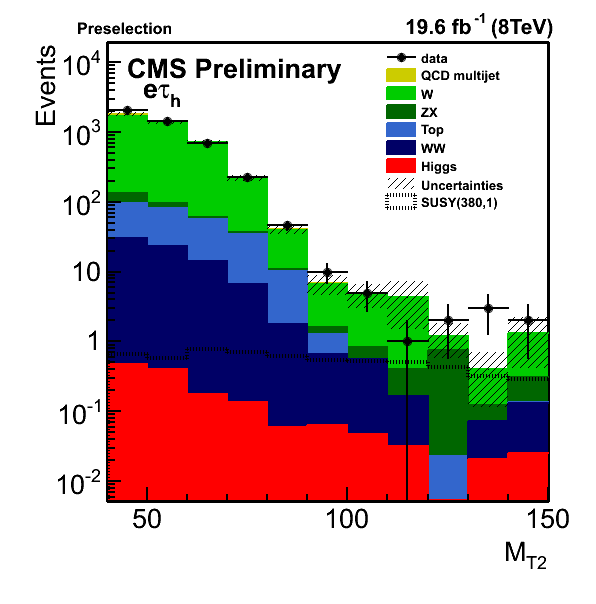
\includegraphics[angle=0,scale=0.375]{SelectionEleTau/MT2_eletau.png}
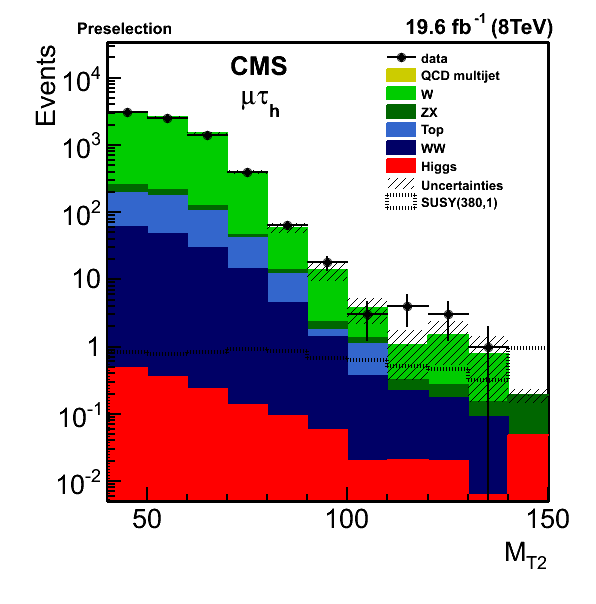
\includegraphics[angle=0,scale=0.375]{SelectionMuTau/MT2_mutau.png}
\caption{\mttwo  distributions for events in the sample after preselection, compared to SM expectation in (left) \eTau and (right) \muTau channels. The signal distribution is shown for $m_{\chione}=380\GeV,~m_{\PSGczDo}=1\GeV$.}
\label{fig:mt2leptontau}
\end{figure}






